\documentclass[11pt,titlepage]{article}

%Laenderspezifische Einstellungen bzgl. Rechtschreibung, Sonderzeichen und Kodierung
\usepackage[utf8]{inputenc}
\usepackage[english]{babel}
\usepackage[T1]{fontenc}
\usepackage{titlesec}
\usepackage{graphicx}
\usepackage{subcaption}

\usepackage{listings}
\usepackage{color}
\usepackage{courier}
\definecolor{light-gray}{gray}{0.85}
\lstset{
language=C++,
numbers=left,
breaklines=true,
backgroundcolor=\color{light-gray},
tabsize=2,
basicstyle=\footnotesize\ttfamily,
frame=single,
inputencoding=utf8,
extendedchars=true,
showstringspaces=false,
literate =
	{ä}{{\"a}}1
	{ö}{{\"o}}1
	{ü}{{\"u}}1
	{Ä}{{\"A}}1
	{Ö}{{\"O}}1
	{Ü}{{\"U}}1
	{ß}{{\ss}}1
	{ₙ}{{$_n$}}1
}

\def\ContinueLineNumber{\lstset{firstnumber=last}}

\usepackage[
	a4paper,
	top = 2cm,
	bottom = 2 cm,
	left = 2cm,
	right = 2cm,
	headheight = 15pt,
	includeheadfoot
	]{geometry}
\usepackage{fancyhdr}
\usepackage{amssymb}
\usepackage{amsmath}
\usepackage[english]{varioref}
\usepackage{hyperref}

\fancypagestyle{firstPage}{
	\fancyhead[LE,RO]{\textsc{Page} \thepage}
	\fancyhead[LO,RE]{}
	\fancyheadoffset[LE,RO]{2.5cm}
	\renewcommand{\headrulewidth}{0.5pt}
	
	\fancyfoot[LE,RO]{\tiny{Assignment 1, Felix Dreßler (k12105003), created: \today}}
	\cfoot{}
	\fancyfootoffset[Le,RO]{2.5cm}
	\renewcommand{\footrulewidth}{0.5pt}
}

\fancypagestyle{fancy}{
	\fancyhead[R]{Page \thepage}
	\fancyhead[L]{\leftmark}
	\renewcommand{\headrulewidth}{1.25pt}

	\fancyfoot[L]{\tiny{Programming 2 - Assignment 1, created: \today}}
	\fancyfoot[R]{\tiny{ Felix Dreßler (k12105003)}}
	\cfoot{}
	\renewcommand{\footrulewidth}{1.25pt}
}

\setlength{\headsep}{10mm}
\setlength{\footskip}{10mm}

\setlength{\parindent}{0mm}
\setlength{\parskip}{1.1ex plus0.25ex minus0.25ex}
\setlength{\tabcolsep}{0.2cm} % for the horizontal padding

\pagestyle{fancy}

\title{Programming 2 - Assignment 1}
\author{Felix Dreßler (k12105003)}
\date{\today} %Erstellungsdatum

\begin{document}
\maketitle
	\section{Testing the Program}
		For testing purposes a series of tests was performed. The program was tested first without the implementation of collisions between different atoms for an fixed input saved in "Input.txt" and random generated atoms.
		Next the program was tested including the implementation of collision between different atoms. This was executed once using the same fixed "Input.txt" and with random generated atoms.
		
		For each test, the text output of the program was recorded, stating the initial values of the atoms. Furthermore, screenshots of the initial-state and the end-state are included.
		\subsection{Tests without atom-collison}
			\subsubsection{Input.txt}
				\begin{figure}[h!]
					\centering
					\begin{subfigure}{.5\textwidth}
						\centering
						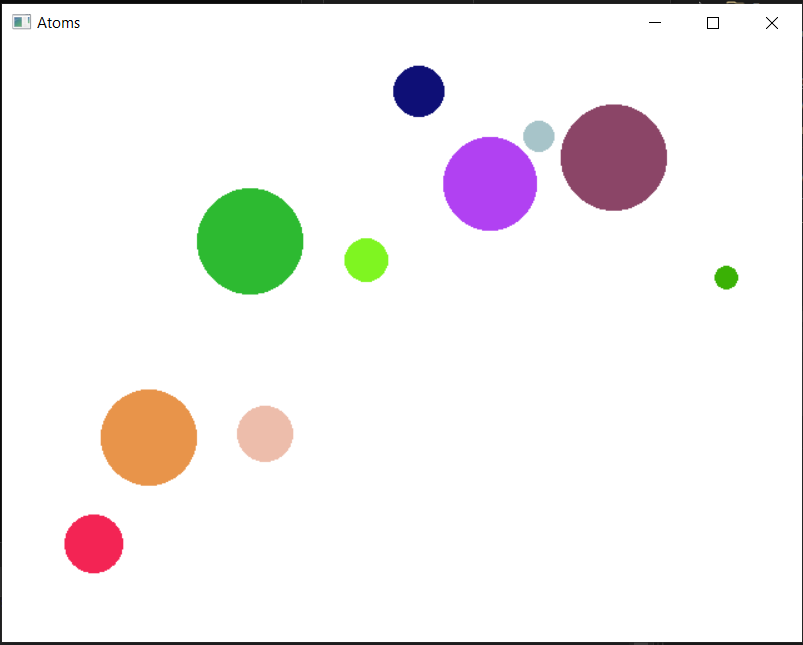
\includegraphics[scale=0.5]{pictures/input_nocollision.png}
						\caption{start state}
						\label{fig:sub1}
					\end{subfigure}%
					\begin{subfigure}{.5\textwidth}
						\centering
						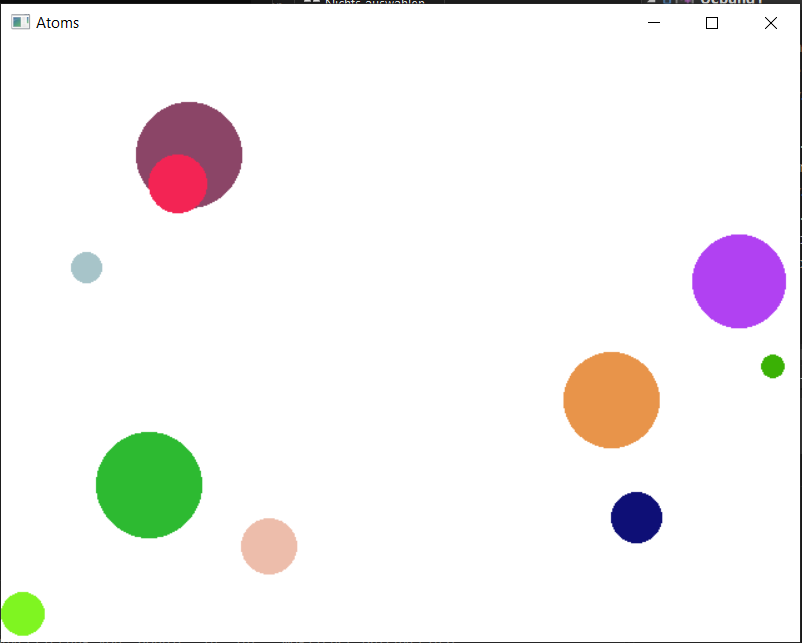
\includegraphics[scale=0.5]{pictures/input_nocollision_final.png}
						\caption{end state}
						\label{fig:sub2}
					\end{subfigure}
				\end{figure}
			\subsubsection{randomly created atoms}
			\begin{lstlisting}[numbers=none]
			the number of Atoms is: 3
			Atom 1 has the following values assigned:
			Color1 is      11200266
			Radius1 is     28
			x Pos.1 is     283
			y Pos.1 is     275
			vx1 is         6
			vy1 is         16
			Atom 2 has the following values assigned:
			Color2 is      3412068
			Radius2 is     28
			x Pos.2 is     169
			y Pos.2 is     142
			vx2 is         17
			vy2 is         7
			Atom 3 has the following values assigned:
			Color3 is      16597665
			Radius3 is     24
			x Pos.3 is     70
			y Pos.3 is     317
			vx3 is         20
			vy3 is         18
			\end{lstlisting}
				\begin{figure}[h!]
					\centering
					\begin{subfigure}{.5\textwidth}
						\centering
						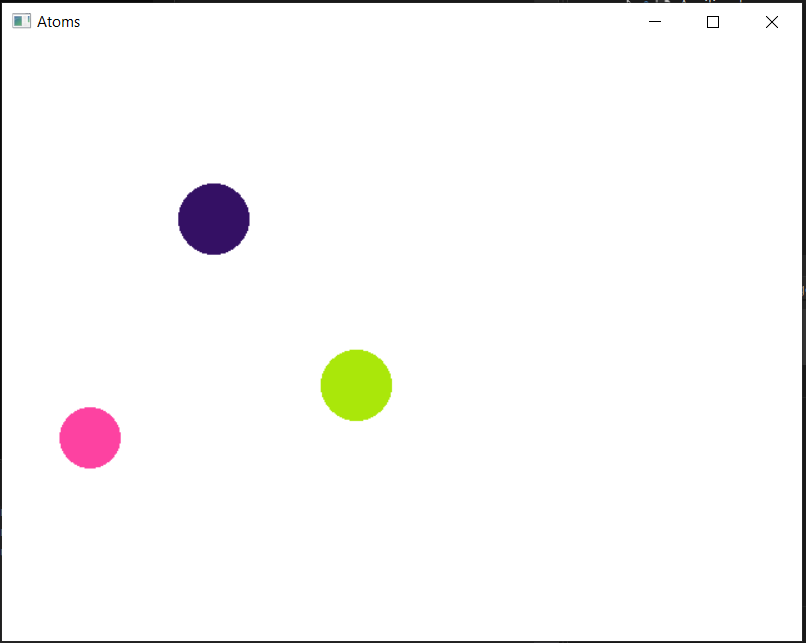
\includegraphics[scale=0.5]{pictures/random_nocollision.png}
						\caption{start state}
					\end{subfigure}%
					\begin{subfigure}{.5\textwidth}
						\centering
						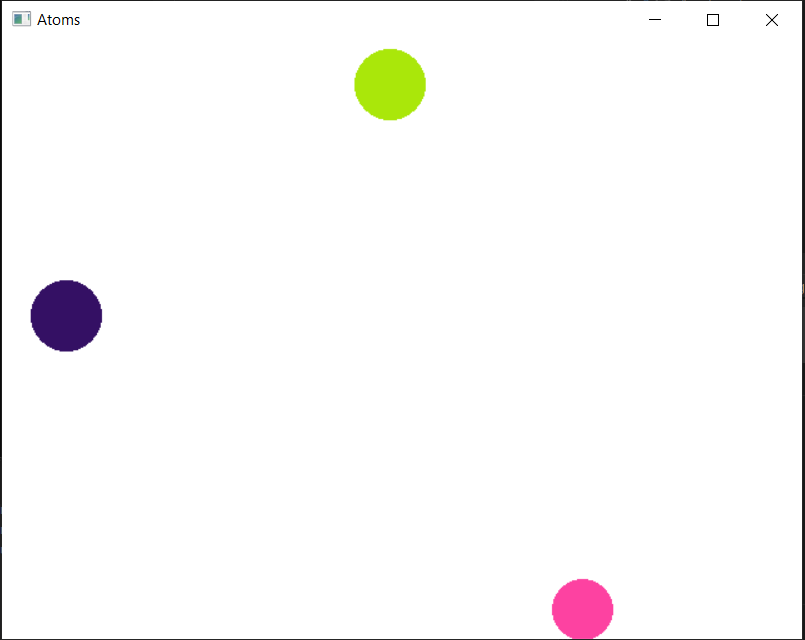
\includegraphics[scale=0.5]{pictures/random_nocollision_final.png}
						\caption{end state}
					\end{subfigure}
				\end{figure}
	
\newpage
		\subsection{Tests with atom-collsion}
			\subsubsection{Input.txt}
				\begin{figure}[h!]
					\centering
					\begin{subfigure}{.5\textwidth}
						\centering
						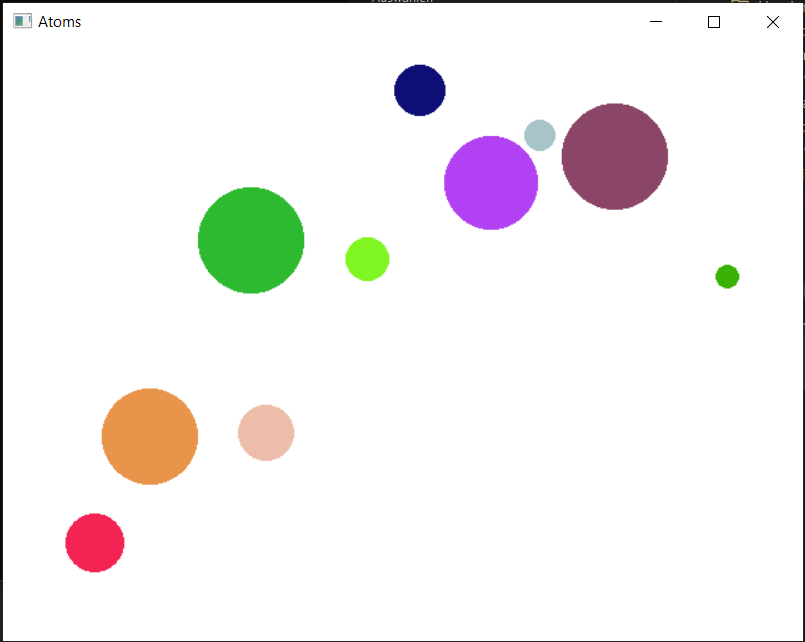
\includegraphics[scale=0.5]{pictures/input_collision.png}
						\caption{start state}
					\end{subfigure}%
					\begin{subfigure}{.5\textwidth}
						\centering
						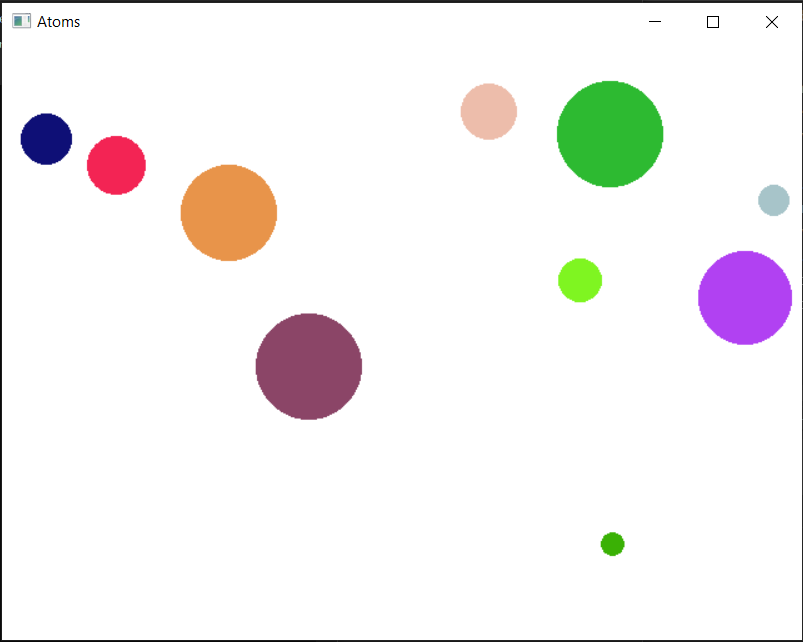
\includegraphics[scale=0.5]{pictures/input_collision_final.png}
						\caption{end state}
					\end{subfigure}
				\end{figure}			
			
			\subsubsection{randomly created atoms}
			Input Data:
			\begin{lstlisting}[numbers=none]
			the number of Atoms is: 3
			Atom 1 has the following values assigned:
			Color1 is      12312020
			Radius1 is     23
			x Pos.1 is     577
			y Pos.1 is     200
			vx1 is         5
			vy1 is         8
			Atom 2 has the following values assigned:
			Color2 is      5024215
			Radius2 is     37
			x Pos.2 is     565
			y Pos.2 is     411
			vx2 is         22
			vy2 is         18
			Atom 3 has the following values assigned:
			Color3 is      6381998
			Radius3 is     26
			x Pos.3 is     328
			y Pos.3 is     327
			vx3 is         7
			vy3 is         17
			\end{lstlisting}
			\begin{figure}[h!]
				\centering
				\begin{subfigure}{.5\textwidth}
					\centering
					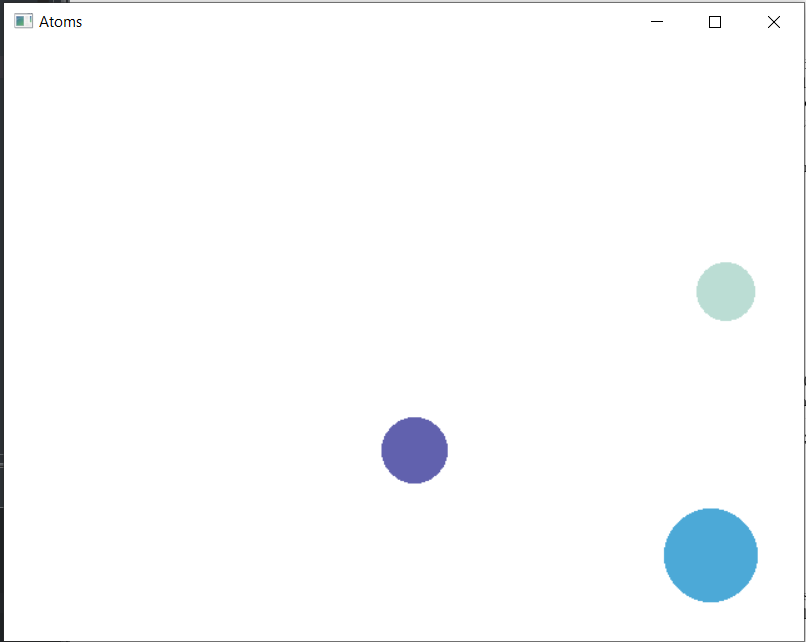
\includegraphics[scale=0.5]{pictures/random_collision.png}
					\caption{start state}
				\end{subfigure}%
				\begin{subfigure}{.5\textwidth}
					\centering
					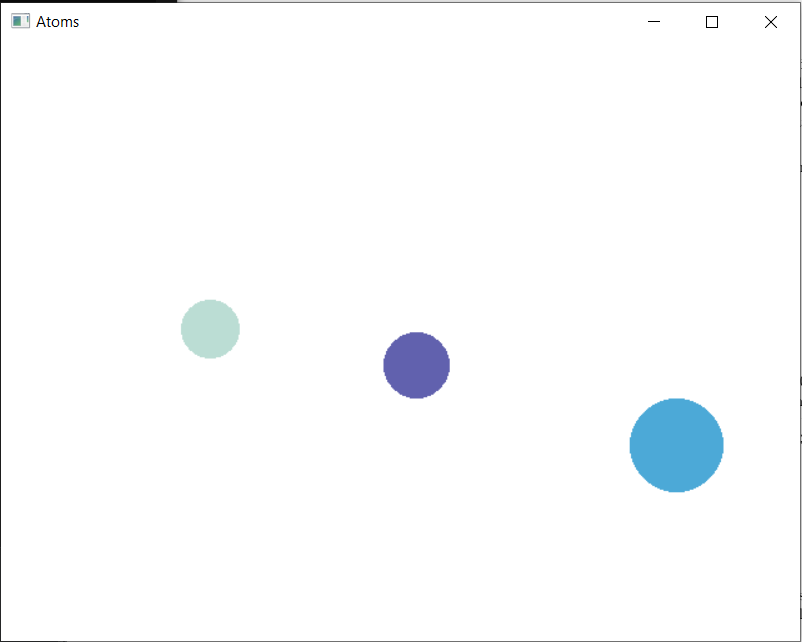
\includegraphics[scale=0.5]{pictures/random_collision_final.png}
					\caption{end state}
				\end{subfigure}
			\end{figure}
						
\newpage			
	\section{The Program - Main.cpp}	
		\subsection{Header of Main.cpp}
			The following paragraph shows the beginning of the File "Main.cpp" of the "Atoms" Project. 
			We see, that in comparison to the given Header in the assignment, there is an "Auxiliary.h" included in line 32. This Header-File will be discussed in the next section.
			
			There are also four global variables defined in lines 34 to 38. W and H are width and height of the created window, in which the atoms will be simulated.
			S describes the time that will pass between each frame. It will be passed to the Sleep function that is describes in lines 14 to 25.
			\lstinputlisting[firstline=0,lastline=38]{Main.cpp}
			
			
		\subsection{structure "Atom"}	
			\ContinueLineNumber
			\lstinputlisting[firstline=40,lastline=61]{Main.cpp}
			
		\subsection{Function "number"}
			\ContinueLineNumber
			\lstinputlisting[firstline=63,lastline=101]{Main.cpp}
			
		\subsection{Function "init"}
			\ContinueLineNumber
			\lstinputlisting[firstline=103,lastline=210]{Main.cpp}
			
		\subsection{Function "Draw"}
			\ContinueLineNumber
			\lstinputlisting[firstline=212,lastline=233]{Main.cpp}
			
		\subsection{Function "Update"}
			\ContinueLineNumber
			\lstinputlisting[firstline=235,lastline=338]{Main.cpp}
			
		\subsection{Main}
			\ContinueLineNumber
			\lstinputlisting[firstline=340,lastline=360]{Main.cpp}
			
\newpage			
		\section{The Program - Auxiliary}
		For better clarity, auxiliary functions were outsourced to the files 
		"Auxiliary.h" and "Auxiliary.cpp".
			\subsection{Auciliary.h}
			In the file "Auxiliary.h", the auxiliary functions are declared.
				\lstset{firstnumber=1}
				\lstinputlisting{Auxiliary.h}
			\subsection{Auxiliary.cpp}
			In the file "Auxiliary.cpp" the auxiliary functions are defined.
			
			"random" creates a random value in between two limits. It may seem unintuitive to implement this function this way, but in order to be able to reach more possible values with bigger given limtits (for example the limits 0 and 0xFFFFFF which are used to represent colours) we would not be able to get any red. This is because the RAND\textunderscore MAX is too low on some common C++ compilers.
				\lstinputlisting{Auxiliary.cpp}
\end{document}